\chapter{Systemarkitektur}\label{kapitel_Systemark}

\begin{longtabu} to \linewidth{@{}l l l X[j]@{}}
    Version &    Dato &    Ansvarlig &    Beskrivelse\\[-1ex]
    \midrule
    0.1 &    4/11-15 &    Alle &    Tilføjelse af arkitektur\\
    Tekst &    Tekst &    Tekst &    Tekst.\\
    Tekst &    Tekst &    Tekst &    Tekst.\\
    Tekst &    Tekst &    Tekst &    Tekst.\\
\label{version_Systemark}
\end{longtabu}

\textbf{Formål}\\
Til beskrivelse af systemarkitekturen og det detaljerede design for produktet, er der benyttet SysML.
SysML anvendes her, da blodtryksmålesystemet både indeholder software og hardware. Et af de  
vigtigste argumenter for brug af SysML er, at de fastlagte standarder i sproget medfører en bedre 
formidling af systemet, hvilket giver et større overblik.


\section{Hardware}
Hardware-delen består af et elektronisk kredsløb, som forstærker signalet fra tryktransduceren og filtrerer det med et indbygget analogt filter.\\
\newline
Til at skabe overblik over blodtryksmålesystemets hardware er der uarbejdet en figur, der viser hele det overordnet system.

\begin{figure}[H]
\centering
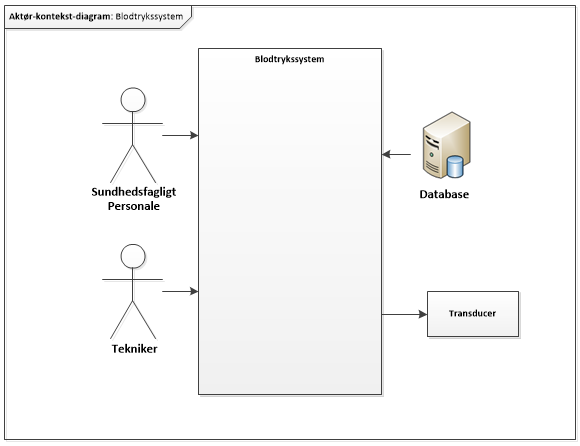
\includegraphics[scale=0.90]{ak.PNG}
\caption{Blodtryksmålersystemet}
\end{figure}

Denne illustrerer, at der ind i transduceren kommer tryk og ud kommer et støjfyldt signal. Dette signal bliver ved forstærkeren forstærket og heraf et forstærket støjfyldt signal. Igennem filtret bliver støjen filtreret fra. Det filtrerede signal føres igennem DAQ’en, som omdanner det til et digitalt signal, som anvendes i computerens softwareprogram.\\
\newline
Til at præcisere komponenterne i blodtryksmålesystemets hardware, er der valgt at lave strukturdiagrammer. Her er der anvendt blokdefinitionsdiagram (BDD) og et internt blokdiagram (IBD).\\
\newline 

\subsection{BDD}
BDD'et er anvendt til, at dokumentere nedbrydningen af systemet og forholdene mellem blokkene. Det interne blokdiagram er anvendt til, at dokumentere den interne struktur i blokkene. 

\textbf{Blokbeskrivelser:}
\begin{itemize}
\item 
\end{itemize}
\subsection{IBD}
\subsubsection{Signalbeskrivelse}

\section{Software}
\subsection{Applikationsmodel}
\subsubsection{Domænemodel}
\subsubsection{Klassediagram}
\subsubsection{Sekvensdiagram}
\subsubsection{Opdateret klassediagram}